\documentclass[
        handout,
        %draft,
        ]{beamer}
\usepackage{amssymb,latexsym,amssymb,amsmath,amsbsy,amsopn,amstext,upgreek}
\usepackage{color,multicol}
\usepackage{graphicx,wrapfig,fancybox,watermark,graphics}
\usepackage{picins}
%\usepackage{emp}
%\usepackage{pstricks,pst-plot}
\usepackage{pgf}
\usepackage{movie15}
\usepackage{hyperref}
\usepackage{pdfpages}
\usepackage{listings,bera}
\definecolor{keywords}{RGB}{255,0,90}
\definecolor{comments}{RGB}{60,179,113}
\lstset{language=C,
keywordstyle=\color{keywords},
commentstyle=\color{comments}\emph}
\hypersetup{
    pdfpagemode=FullScreen, % show in full screen?
}
\usepackage{algorithm}
\usepackage{algorithmic}
\renewcommand{\algorithmicrequire}{\textbf{Input:}}
\renewcommand{\algorithmicensure}{\textbf{Output:}}
% reference entry
\usepackage{bibentry, natbib}
% reference style
\bibliographystyle{IEEEtran} 
%reference lib
\nobibliography{refs}

\usepackage[
	%compress,
	minimal,
	%nonav,
	red,
	%gold,
	%numbers,
	%nologo,
	polyu,
	]{beamerthemeHongKong}
\usefonttheme[professionalfonts]{serif}

\title[Tutorial 11]{Tutorial 11: homework 5 graphs}
\author[COMP210]{Qu Xiaofeng\texorpdfstring{, Teaching Asistant\\\tiny{quxiaofeng.at.polyu@gmail.com, PQ702}}{}}
\institute{COMP210\\Discrete Structure}
\date{\today}

\begin{document}

\titlepage

\section*{Table of Contents}
    \begin{frame}{\secname}
        \tableofcontents
    \end{frame}

\section{Graphs}
    \subsection{Problem 11.1}
        \begin{frame}[c]{\subsecname}
                \begin{figure}
                    \centering
                    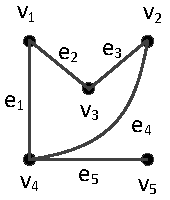
\includegraphics[width=28.6mm]{tut11p10}
                \end{figure}
        \end{frame}
    \subsection{Problem 11.2}
        \begin{frame}[c]{\subsecname}
                \begin{figure}
                    \centering
                    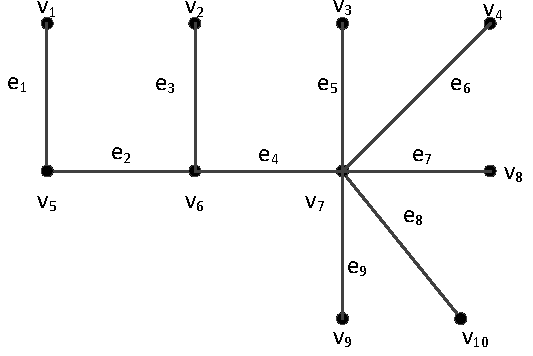
\includegraphics[width=90mm]{tut11p10_2}
                \end{figure}
        \end{frame}
    \subsection{Problem 14}
        \begin{frame}[c]{\subsecname}
                \begin{figure}
                    \centering
                    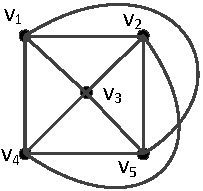
\includegraphics[width=34mm]{tut11p13_1}
                \end{figure}
        \end{frame}
    \subsection{Problem 19}
        \begin{frame}[c]{\subsecname}
            \begin{figure}
                \centering
                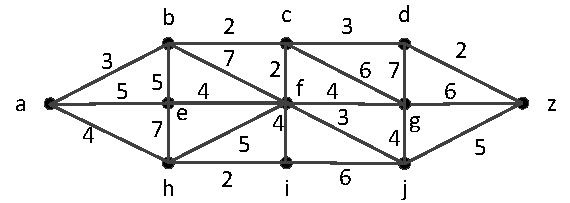
\includegraphics[width=96.3mm]{tut11p17_1}
            \end{figure}
        \end{frame}
    \subsection{Problem 26.1}
        \begin{frame}[c]{\subsecname}
            \begin{figure}
                \centering
                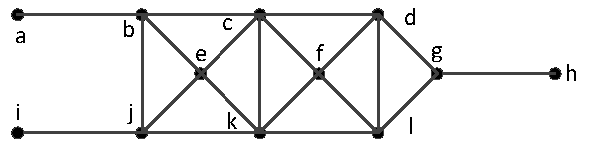
\includegraphics[width=99.6mm]{tut11p23_1_1}
            \end{figure}
        \end{frame}
    \subsection{Problem 26.2}
        \begin{frame}[c]{\subsecname}
            \begin{figure}
                \centering
                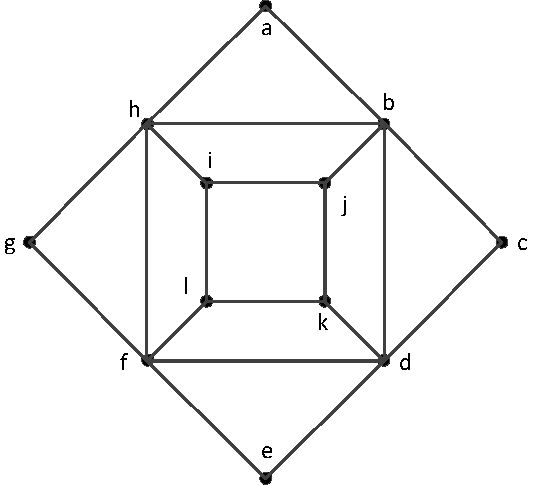
\includegraphics[width=88mm]{tut11p23_2_1}
            \end{figure}
        \end{frame}
\end{document}



